\begin{surferIntroPage}{Tutorial}{tutorial_koord1}{الخطوات الأولى مع SURFER}
يُدعى هذا البرنامج \textenglish{SURFER}. عند قراءة هذه الكلمة، تفكرون على الأرجح بالبحر والشمس والأمواج. ولكن في هذه الحالة، تأتي هذه الكلمة من \textenglish{\it surface} أي سطح بالإنجليزية.
\\
مع برنامج \textenglish{SURFER}، يمكن عرض سطوح وبالتحديد سطوح جبرية. تجدون في هذا البرنامج التعليمي شرحاً لماهية السطوح الجبرية. يمكنكم إختيار سطحاً معروضاً على اليمين من أجل تصفح فصول هذا البرنامج التعليمي.\\
يشكل \textenglish{SURFER} جزءاً من معرض إيماجينيري
 \textenglish{(IMAGINARY)}
  المتنقل الذي بدأ في 2008 بمناسبة السنة الألمانية للرياضيات . هذا المعرض هو مشروع قام به معهد أوبرفولفاك لأبحاث الرياضيات
\textenglish{(Mathematisches Forschungsinstitut Oberwolfach)}
 الواقع في الغابة السوداء في ألمانيا. في كل اسبوع، تقوم في المعهد ورشات دراسية حول مواضيع أخيرة في أبحاث الرياضيات. هذه الورشات الدراسية مهمة لتعزيز حديثة بين العلماء حول العالم. \\
\vspace{0.2cm} \hspace{3.5cm}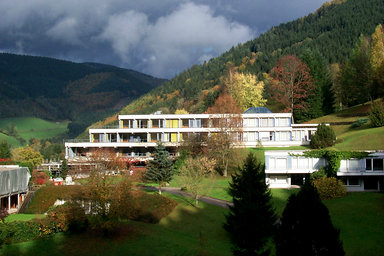
\includegraphics[width=3cm]{./../../common/images/photo_mfo.jpg}\\
يمكن تنزيل برنامج \textenglish{SURFER} مجاناً من صفحتنا الرئيسية: \\
\begin{centering}
\textenglish{www.imaginary.org}\\
\end{centering}
 \vspace{0.2cm}
على اليمين، يمكن إختيار إحدى الصفحات التعليمية بدءاً بسطح زيتروس
 \textenglish{(Zitrus)}.
  على اليسار، يمكن الإنتقال إلى جاليريات أخرى مثل جاليرية السطوح الإبداعية.
\end{surferIntroPage}
